
\subsubsection{Analyzing fingerprinting API presence in Browsers}
We wanted to answer two different questions regarding to browser fingerprinting in our paper. Are browsers becoming more fingerprintable as the time goes by? Can we also say that all browsers are fingerprintable?

Now that we have collected these fingerprinting APIs list, we try to examine different browser versions and see how many of these APIs are active in various browser versions.
We analyzed the presence of these APIs in every browser version in our analysis. For Chrome, we observe that Chrome 49, which is the youngest Chrome browser version in our analysis, has 139 fingerprinting APIs which is the smallest number among other versions.
On the other hand, Chrome 81, which is the latest Chrome browser in our analysis, has 274 fingerprinting APIs in it, which is the biggest number among other Chrome versions. So, it is obvious that Chrome is having more fingerprinting APIs in its newer versions and creating a unique fingerprint for the user is becoming easier in this browser. 
For Firefox, we figure out that the least number of APIs exist in Firefox 45 which is the youngest Firefox version in our study. The latest Firefox version which is Firefox 75 has 271 fingerprinting APIs in it but it is not the biggest number. Firefox 60 through 71 have 276 APIs which is the biggest number of APIs among other Firefox versions. It seems that fingerprinting APIs are being reduced in the latest versions of Firefox but newer versions are having much more features compared to the earlier versions.

In Figure \ref{fig:fingerprint-apis} we present the detailed information about presence of fingerprinting APIs in different browser versions. As we look through the graph, we realize that in January 2017, we have a significant increase in the number of fingerprinting APIs. More than 100 fingerprinting APIs are added to both of these browsers after this period. In order to find out what has happened to the browsers in that period of time, we looked through the release notes for both Firefox 51~\cite{firefox-51-notes} and Chrome 56~\cite{chrome-56-notes} to find out the root cause of this unpleasant event. 

Looking through the release notes, we find out that in Google Chrome 56, HTML5 has been enabled for all users by default. This change disabled Adobe Flash Player and from this time, user's permision was needed for websited to run Flash. They also enabled WebGL 2.0 API which provides a new rendering context and supports objects for the HTML5 Canvas elements. This context allows rendering using an API that conforms closely to the OpenGL ES 3.0 API~\footnote{https://www.khronos.org/registry/webgl/specs/latest/2.0/}. These are not every feature that have been introduced in Chrome 56 but are the major ones. In Firefox 51, we observe that they have also added support for WebGL2 and some more features.

When we look into our fingerprinting APIs list, we see that 107 fingerprinting APIs are related to \texttt{WebGL2RenderingContext} which was added to Firefox 51 and Chrome 56. This explains the spike in the number of fingerprinting APIs in January 2017 which is the release date of Chrome 56 and Firefox 51. 

\begin{figure*}[ht]
    \centering
    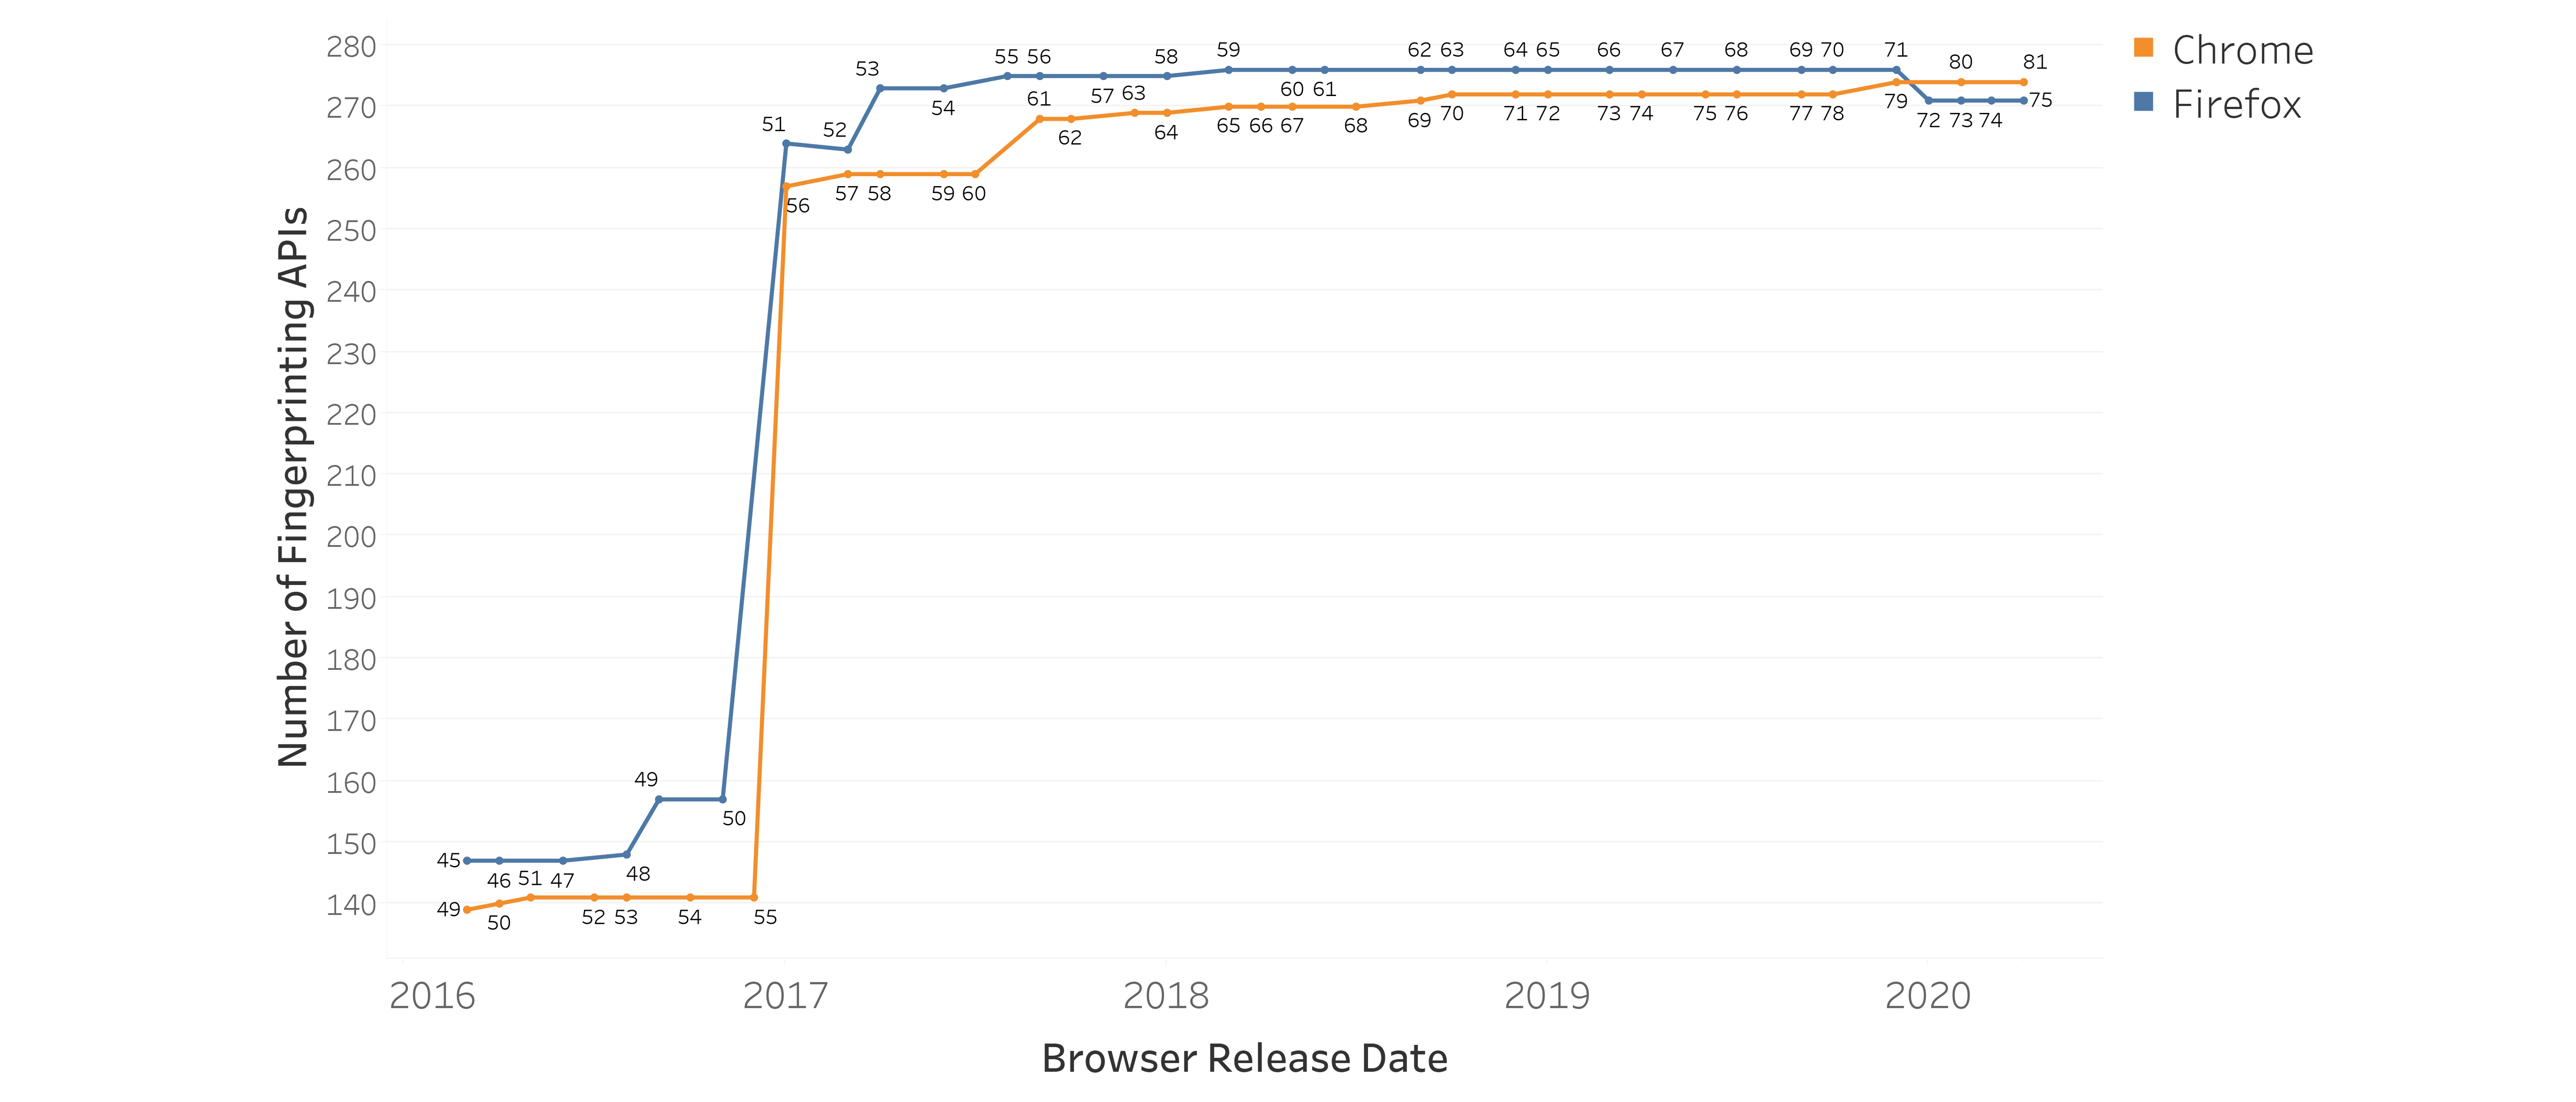
\includegraphics[width=\textwidth]{figures/Fingerprinting-APIs.png}
    \caption{Presence of Fingerprinting APIs among different browser versions. The orange line shows Google Chrome versions while the Blue line represents Firefox versions. The X-axis shows browser release date and the Y-Axis shows number of fingerprinting APIs.}
    \label{fig:fingerprint-apis}
\end{figure*}

\subsubsection{Unique Feature Set}
We created a feature set for each browser version that we had.
A feature set is a set of browser features that exist in a specific browser version.
After creating the feature set for each browser version in our study, we compared these sets to each other and realized that all of these sets are unique.
This means that there are no two browsers that have the same feature set which supplements our hypothesis that all browsers are fingerprintable. The presence of temporary and non-persistent features lead to this difference in feature sets among browsers. Vendors keep removing and adding features to their newer versions so that the feature set for each version is unique and different from the others.

One other observation of our study is that vendors especially Google Chrome are adding lots of features to their newer versions but they do not remove features as much as they add. We define a set called unique feature set as the set of features that make a specific browser version unique; either by existing in the feature set of that browser or by not being in the feature set. We generate the unique feature set for every browser in our study and see that this set is getting smaller over time in newer versions. Thus, we can say that the feature set for newer browsers is becoming more similar and they have much more intersection with each other compared to the older ones. So the feature set for browsers is converging and we are tending to the homogeneity of browser features. 

